\documentclass[english,11pt,letterpaper,onecolumn]{scrartcl}

%\usepackage[utf8]{inputenc}
\usepackage{babel}
\usepackage{csquotes}
\usepackage{amsmath}
\usepackage{amsfonts}
\usepackage{mathptmx}
\usepackage{enumitem}
% Extra leading.
\renewcommand{\baselinestretch}{1.125}
\usepackage{tocloft}
% \usepackage{fancyhdr}
\usepackage{scrlayer-scrpage}
\usepackage{ifthen}
\usepackage{keyval}
\usepackage{geometry}
\usepackage{url}
\usepackage{calc}
\usepackage{array}
\usepackage{graphicx}
\usepackage{color}
\usepackage{listings}
\usepackage{supertabular}
% definitions used by included articles, reproduced here for
% educational benefit, and to minimize alterations needed to be made
% in developing this sample file.
\usepackage{amssymb}
\usepackage{latexsym}
\usepackage{amsfonts}
\usepackage{amsmath}
\usepackage{amscd}     % commutative diagrams
\usepackage{mathrsfs}  % This package allows the use of script letters. Type \mathscr to invoke math script.
\usepackage{amsbsy}
%\usepackage{scrpage2}
\usepackage[pdftex,
colorlinks=true,
linkcolor=blue,
pdfpagelabels,
pdfstartpage=3
]{hyperref}
% \usepackage{poemscol}
% \global\verselinenumbersfalse
\makeindex
\definecolor{LstColor}{cmyk}{0.1,0.1,0,0.025}
\setcounter{tocdepth}{9}
\newcommand\floor[1]{\lfloor#1\rfloor}
\newcommand\ceil[1]{\lceil#1\rceil}
\usepackage{lmodern}
\usepackage{amssymb,amsmath}
\usepackage{ifxetex,ifluatex}
\hypersetup{breaklinks=true,
bookmarks=true,
pdfauthor={},
pdftitle={},
colorlinks=true,
citecolor=blue,
urlcolor=blue,
linkcolor=magenta,
pdfborder={0 0 0}}

\usepackage{amsfonts}
\usepackage{amsmath}
\usepackage{amssymb}
\usepackage{graphicx}

\usepackage{version}%
\setcounter{MaxMatrixCols}{30}

%%%% Packages added - Peter
\usepackage{color}
\usepackage{amscd}     % commutative diagrams
\usepackage{mathrsfs}  % This package allows the use of script letters.
%%%%%%%%%%%%%%%%%%%%%%%%%%%%%%%%%%%%%%%%%%%%%%%%%%%%%

\newtheorem{theorem}{Theorem}[section]
%\theoremstyle{plain}
\newtheorem{acknowledgement}{Acknowledgement}
\newtheorem{algorithm}{Algorithm}[section]
\newtheorem{axiom}{Axiom}[section]
\newtheorem{case}{Case}[section]
\newtheorem{claim}{Claim}[section]
\newtheorem{conclusion}{Conclusion}[section]
\newtheorem{condition}{Condition}[section]
\newtheorem{conjecture}{Conjecture}[section]
\newtheorem{corollary}{Corollary}[section]
\newtheorem{criterion}{Criterion}[section]
\newtheorem{definition}{Definition}[section]
\newtheorem{example}{Example}[section]
\newtheorem{exercise}{Exercise}[section]
\newtheorem{lemma}{Lemma}[section]
\newtheorem{notation}{Notation}[section]
\newtheorem{problem}{Problem}[section]
\newtheorem{proposition}{Proposition}[section]
\newtheorem{remark}{Remark}[section]
\newtheorem{solution}{Solution}[section]
\newtheorem{summary}{Summary}[section]
\numberwithin{equation}{section}
\excludeversion{comment1}

%%%%% Macros added - Peter
\newcommand{\st}{\,|\,}
\newcommand{\C}{\mathbb{C}}
\newcommand{\F}{\mathbb{F}}
\newcommand{\I}{\mathbb{I}}
\newcommand{\bH}{\mathbb{H}}
\newcommand{\K}{\mathbb{K}}
\newcommand{\N}{\mathbb{N}}
\newcommand{\Q}{\mathbb{Q}}
\newcommand{\R}{\mathbb{R}}
\newcommand{\T}{\mathbb{T}}
\newcommand{\X}{\mathbb{X}}
\newcommand{\Y}{\mathbb{Y}}
\newcommand{\Z}{\mathbb{Z}}
%
\newcommand{\cB}{\mathcal{B}}
\newcommand{\cC}{\mathcal{C}}
\newcommand{\mcD}{\mathcal{D}}
\newcommand{\cE}{\mathcal{E}}
\newcommand{\cF}{\mathcal{F}}
\newcommand{\cG}{\mathcal{G}}
\newcommand{\calH}{\mathcal{H}}
\newcommand{\cJ}{\mathcal{J}}
\newcommand{\cK}{\mathcal{K}}
\newcommand{\mcL}{\mathcal{L}}
\newcommand{\cM}{\mathcal{M}}
\newcommand{\cN}{\mathcal{N}}
\newcommand{\cO}{\mathcal{O}}
\newcommand{\calR}{\mathcal{R}}
\newcommand{\cS}{\mathcal{S}}
\newcommand{\mcT}{\mathcal{T}}
\newcommand{\cU}{\mathcal{U}}
\newcommand{\cW}{\mathcal{W}}
\newcommand{\cY}{\mathcal{Y}}
\newcommand{\bcF}{\boldsymbol{\mathcal{F}}}
%
\newcommand{\oY}{\overline{Y}}
\newcommand{\uY}{\underline{Y}}
%
\renewcommand{\Re}{\mathop{\mathrm{Re}}}
\renewcommand{\Im}{\mathop{\mathrm{Im}}}
%
\newcommand{\card}{\mathop{\mathrm{card}}}
\newcommand{\Int}{\mathop{\mathrm{int}}}
\newcommand{\eps}{\varepsilon}
\newcommand{\kap}{\varkappa}
\newcommand{\be}{\begin{equation}}
\newcommand{\ee}{\end{equation}}
\newcommand{\inn}[2]{{\langle #1,#2 \rangle}}
\newcommand{\wt}[1]{{\widetilde{#1}}}

\newcommand{\conv}{\mathrm{conv}\,}
\newcommand{\bx}{{\boldsymbol{x}}}
\newcommand{\by}{{\boldsymbol{y}}}
\newcommand{\bk}{{\boldsymbol{k}}}
\newcommand{\bm}{{\boldsymbol{m}}}
\newcommand{\bc}{{\boldsymbol{c}}}
\newcommand{\ba}{{\boldsymbol{a}}}
\newcommand{\bp}{{\boldsymbol{p}}}
\newcommand{\bP}{{\mathbb{P}}}
\newcommand{\bS}{{\boldsymbol{S}}}
\newcommand{\bq}{{\boldsymbol{q}}}
\newcommand{\bfe}{{\boldsymbol{e}}}
\newcommand{\bone}{{\boldsymbol{1}}}
\newcommand{\bu}{{\boldsymbol{u}}}
\newcommand{\bv}{{\boldsymbol{v}}}
\newcommand{\bw}{{\boldsymbol{w}}}
\newcommand{\bff}{{\boldsymbol{f}}}
\newcommand{\bkk}{{\boldsymbol{k-1}}}
\newcommand{\bxi}{{\boldsymbol{Xi}}}
\newcommand{\balpha}{{\boldsymbol{\alpha}}}
\newcommand{\bbeta}{{\boldsymbol{\beta}}}
\newcommand{\bgamma}{{\boldsymbol{\gamma}}}
\newcommand{\blambda}{{\boldsymbol{\lambda}}}
\newcommand{\bmu}{{\boldsymbol{\mu}}}
\newcommand{\gr}{{\mathrm{graph\,}}}
\newcommand{\of}{\overline{f}}
\newcommand{\og}{\overline{g}}
\newcommand{\oc}{\overline{c}}
\newcommand{\ou}{\overline{u}}
\newcommand{\ox}{\overline{x}}
\newcommand{\oX}{\overline{X}}
\newcommand{\oXi}{\overline{X}_i}
\newcommand{\uc}{\underline{c}}
\newcommand{\oy}{\overline{y}}
\newcommand{\uy}{\underline{y}}
\newcommand{\odelta}{\overline{\delta}}
\newcommand{\udelta}{\underline{\delta}}
\newcommand{\oPhi}{\overline{\Phi}}
\newcommand{\map}{\textrm{Map}\,}
\newcommand{\loc}{\mathrm{loc}}
\newcommand{\mydot}{\;\cdot\;}
\DeclareMathOperator{\dom}{dom}
\DeclareMathOperator{\range}{range}
\DeclareMathOperator{\id}{id}
\DeclareMathOperator{\Aff}{Aff}
\DeclareMathOperator{\GL}{GL}
\DeclareMathOperator{\diag}{diag}

\usepackage[
backend=biber,
bibencoding=utf8,
style=numeric,
sorting=ynt,
hyperref=true,
backref=true
]{biblatex}
\addbibresource{gogins.bib}
\begin{document}

\title{Parametric Composition in Score Spaces with Harmony} \author{Michael
Gogins \\ \texttt{michael.gogins@gmail.com}} \maketitle
%\pagestyle{scrheadings}

\begin{abstract}
Extending our earlier work on iterated function systems (IFS) music, we present
new methods for using IFS to generate scores in spaces with \emph{harmony},
where each point in the space specifies not only a pitch, a time, and perhaps
other properties, but also an interval, chord, or scale to which that pitch
belongs. As before, we generate scores as the attractors of IFS. However, here
we construct the Hutchinson operators for generating these attractors such that,
in the time-harmony planes of the score space, the attractor is the graph of a
function of time, using the mathematics of fractal interpolation functions
(FIFs) and the Read-Bajraktarevi\'c operator. In the other planes of the score
space, the attractor may take any form. This helps to ensure that the composer
and listener will hear the harmony as a linear progression through time, while
permitting more complex transformations in other dimensions of the score. The
Collage Theorem proves that any score may be approximated, as closely as
desired, by such an IFS. One method of composing is then to manually construct
these IFS, or to evolve them using the genetic algorithm, and then to render the
IFS to an actual score. Additionally, one complex virtual parameter can be
derived to represent each set (potentially dozens or more numbers) of the IFS
parameters used to compute each score graph. Each virtual parameter may be
mapped to the score produced from the corresponding IFS, thus producing a
parametric map of scores colored by some musical feature of interest. Other
methods of composition are then to interactively explore such parametric maps,
or to interpolate between two scores located in such a map.
\end{abstract}

%\lohead{Parametric Composition}

\section{Introduction}

\lstset{language=c++,basicstyle=\ttfamily\tiny,commentstyle=\ttfamily\tiny,tabsize=2,breaklines,backgroundcolor=\color{LstColor},fontadjust=true,keepspaces=false,showstringspaces=false,moredelim=[is][\textbf]{\\emph\{}{\}}}

In general, we define a \textit{score space} as a space in which a set of points
represents a piece of music, \textit{e.g.}\ notes on the grand staff, punches in
a piano roll, some more abstract space, or even grains of sound on a sonogram.
We define a \textit{score generator} as a computer program that generates a
musical score in some score space. We define a \textit{parametric score
generator} as one whose behavior is completely defined by numerical parameters.

Then \textit{parametric composition} is the art of composing music by exploring
the parameter space of some parametric score generator. Such exploration can be
performed by literally zooming around in a colored map of the parameter space,
by interpolating between two parameter points in that space, or by evolving
parameters using the genetic algorithm.

We have previously investigated parametric composition in spaces that directly
represent either sound, \textit{e.g.}\ in the form of a grid of sound grains
(Gabor transform) \cite{obsessed}, or scores, \textit{e.g.}\ in the form of a
grid of notes (piano roll) \cite{ifsmusic}.

Here, we extend that work by generating scores in a special score space
constructed from time and the basic symmetries of chord space identified by
Callender, Quinn and Tymoczko \cite{callender:346}, along with pitch, loudness,
and other properties. The dimensions of this score space are: time $t$, set
class (the most basic form of a chord) $P$ (\textit{i.e.}, Callender \textit{et
al.}'s $OPTIC$), inversion $I$, and transposition $T$. Dimensions $t$, $P$, $I$,
and $T$ defines the time-harmony planes, or the basis of a harmony subspace of
the score space. The other dimensions are $k$ pitch as real-valued MIDI numbers,
$v$ loudness as real-valued MIDI velocity numbers, and instrument as real-valued
MIDI channel numbers.

The score generators used here are \textit{iterated function systems} (IFS)
\cite{barnsley1985iterated, 10.2307/24893080, fractalseverywhere}. More
particularly, our score generators are special IFS where the contractive
transformations that make up the IFS are constrained (within the harmony
subspace only) such that the IFS computes attractors that closely approximate
the graphs of functions. The function for such a graph is called a
\textit{fractal approximation} (FA) or fractal interpolation function (FIF), or
simply a \textit{fractal function} \cite{Barnsley1986, fractalseverywhere,
navascues2014fractal}. (It is interesting that all continuous functions are
fractal functions \cite{2016arXiv161001369B}.) One motivation for using this
space to compose is that different points in the harmony subspace are clearly
audible as harmonic differences. Another motivation is that we can use fractal
interpolation within the harmony subspace to ensure that, at any one point in
time, there is one and only one harmony, although of course it may consist of
any number of pitch-classes.

An IFS may be completely specified as a set of numerical parameters. Thus, any
piece of note-based music may be approximated as closely as desired by a fixed
size set of numerical parameters. Although there might be dozens or hundreds of
numbers in such IFS parameters, each parameter set can effectively be
represented as a single real or complex number by using a recursive indexing
scheme. We call this number the \textit{effective parameter} of the IFS because
the complete set of parameters can be recovered (given sufficient numerical
precision) by decoding the index.

Then, using the effective parameters, it is straightforward (if perhaps
compute-intensive) to render a parametric map of all pieces within a given range
of FAs, or to interpolate between two pieces by interpolating between their
effective parameters. It is also, of course, possible to evolve pieces using the
genetic algorithm on sets of actual parameters.

The remainder of this paper develops the mathematical background in somewhat
more detail; discusses the implementation of IFS, indexes for parameters, and
the genetic algorithm for IFS parameters in the Silencio library for algorithmic
composition in JavaScript; and finishes with examples of each of the three
methods of algorithmic composition, implemented in Silencio and Csound.

\section{Mathematical Development}

This section is not intended as a complete, self-contained exposition but rather
as providing entry points for readers who have some exposure to mathematical
music theory or fractal geometry. We have tried to supply references not only to
original publications of ideas, but also to recent reviews or summaries.

\subsection{Chord Spaces}

A \textit{chord space} is simply a space in which each voice of a chord is
represented by a different dimension. A single voice is represented by a point
on a line; an interval, by a point on a plane; a triad, by a point in a
3-dimensional space; and so on. Here the octave is always 12, so that
pitch-classes in 12 TET are always integers (and compatible with MIDI). Chord
space has many uses. For example, Tymoczko \cite{tymoczko2006geometry,
tymoczko2011geometry} showed that perceptually smoother voice-leadings between
chords are represented by shorter distances in chord space.

Even unschooled musicians are aware that pitches transposed to different octaves
are somehow the same. This is expressed in music theory by saying that
pitch-classes, \textit{e.g.} C or F\#, are pitches under \textit{octave
equivalence}. Octave equivalence transforms the line of pitch into a circle, an
\textit{orbifold} or \textit{quotient space} $\mathbb{R}/12$, by gluing the
lowest pitch under octave equivalence to the same pitch an octave higher. There
are other implicitly familiar equivalence classes in music:
\textit{permutational equivalence} (a triad is somehow the same whether the
voices are assigned to violin, trumpet, and flute or to flute, trumpet, and
violin), \textit{cardinality equivalence} (a chord is somehow the same if voices
are doubled in different octaves), and so on. Callender, Quinn, and Tymoczko
\cite{callender:346} have concisely analyzed these equivalence classes, or
symmetries, as different quotients of chord space. Figure \ref{fig:opc} shows
their $OPC$ orbifold $\left(\mathbb{R}/12\mathbb{Z}\right)^{n}/\mathcal{S}_{n}$
(octave, permutational, and cardinality equivalence) for trichords in 12-tone
equal temperament. In all cases $n$ is the the number of voices, and
$\mathcal{S}$ is the symmetry group. $OPC$ is what musicians commonly mean by
``chord.''

\begin{figure}
\centerline{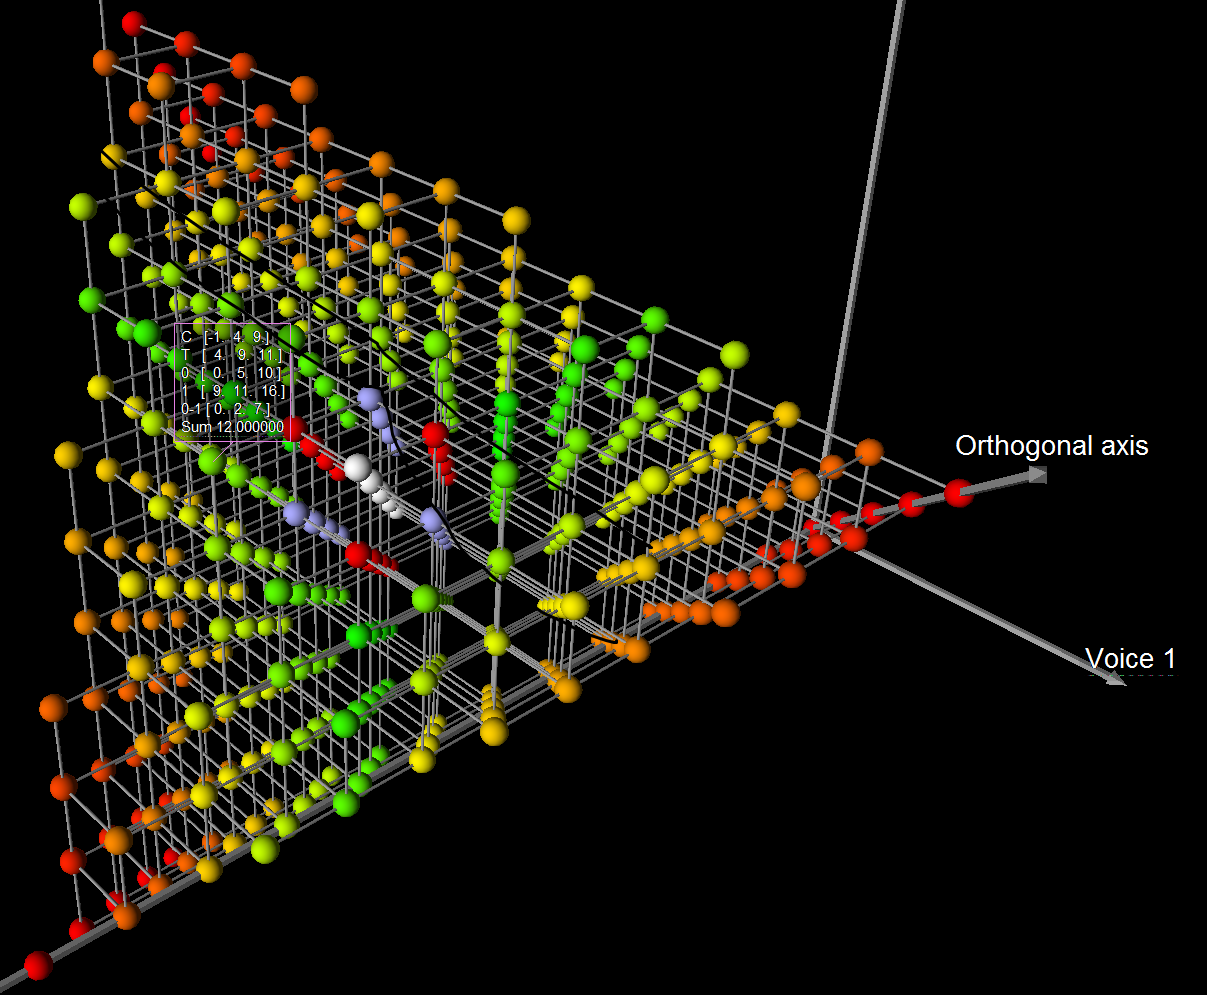
\includegraphics[width = 0.9\textwidth]{opc}}
\caption{\label{fig:opc}
  $OPC$ for trichords in 12TET.}
\end{figure}

If in addition transpositional equivalence is assumed, the orbifold collapses to
a single layer $\left(\mathbb{R}/12\mathbb{Z}\right)^{n-1}/\mathcal{S}_{n}$, in
which points at 120 degrees rotation are equivalent (Figure \ref{fig:opttc}; to
simplify the view, pitches are rounded by semitone). This is $OPTC$, which is
what musicians normally mean by ``chord type.''

\begin{figure}
\centerline{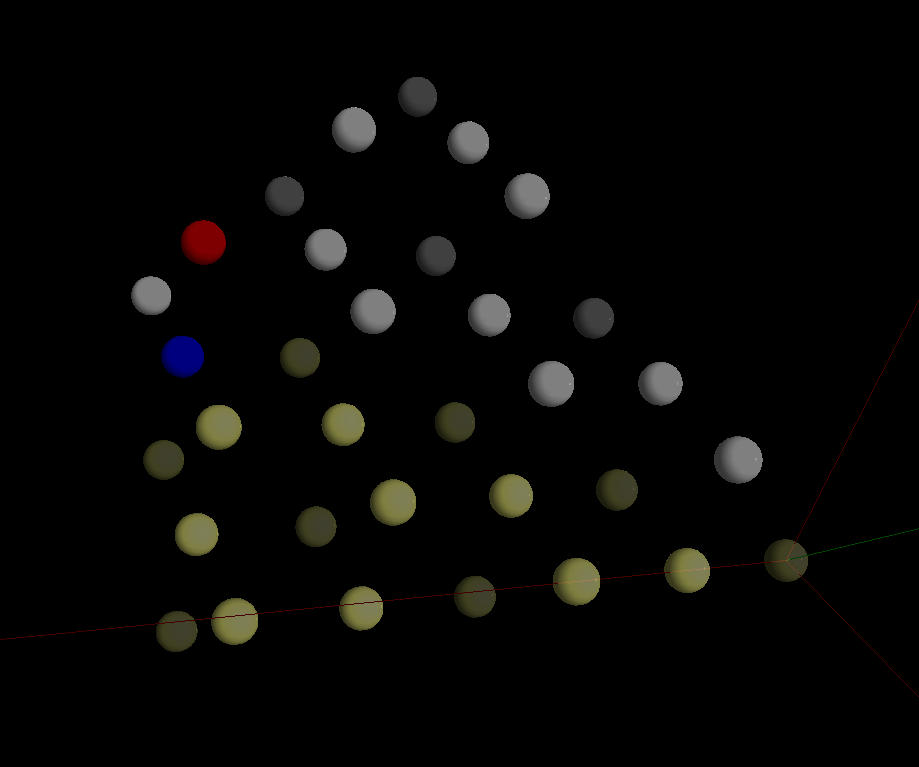
\includegraphics[width = 0.5\textwidth]{opttc}}
\caption{\label{fig:opttc}
  $OPTC$ for trichords in 12TET.}
\end{figure}

A little more theoretical sophistication reveals \textit{inversional
equivalence}: a major triad is somehow the same as a minor triad. The orbifold
folds over or reflects to equate major and minor
$\left(\mathbb{R}/12\mathbb{Z}\right)^{n-1}/(\mathcal{S}_{n} \times
\mathbb{Z}_{2})$ (Figure \ref{fig:optic}; again, rounded by semitone). This is
$OPTIC$, which is what theorists mean by ``set class,'' and is the most abstract
commonly used concept of what is a ``chord.''

\begin{figure}
\centerline{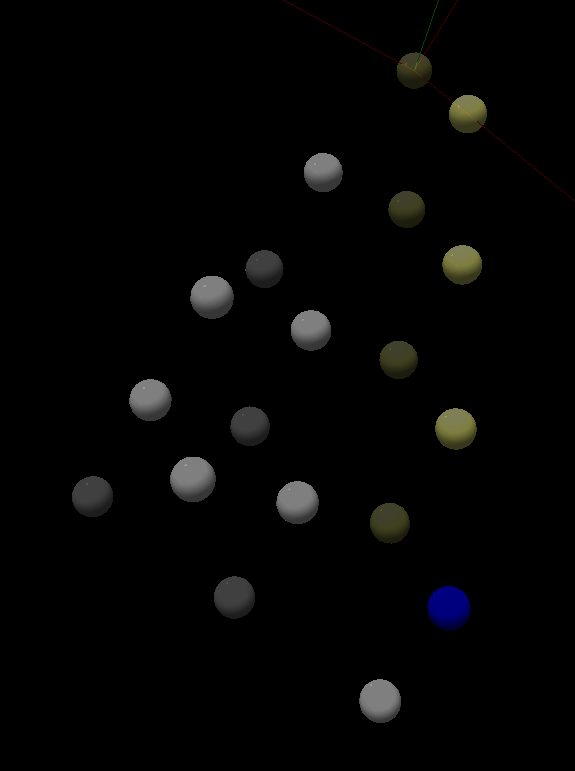
\includegraphics[width = 0.25\textwidth]{opttic}}
\caption{\label{fig:optic}
$OPTIC$ for trichords in 12TET.}
\end{figure}

Here, we do not directly use chord space for composing. Rather, we construct a
space in which each of the irreducible symmetries of chords identified by
Callender, Quinn, and Tymoczko is a separate dimension. We define the semitone
as the generator of transposition, thus making this space discrete (and modeling
12 TET). Then the group elements of each symmetry can be given integer indexes.
These dimensions are:

\begin{description}
\item[$P$] Set class (Callender, Quinn, and Tymoczko's $OPTIC$), the
most abstract conception of a chord; all major and minor triads are equivalent.
The number of elements in P depends upon the maximum number of voices and the
number of divisions of the octave.
\item[$I$] Inversion (reflection by the origin).
\item[$T$] Transposition \emph{modulo} the octave.
\end{description}

\noindent We supplement this chord symmetry space with additional dimensions:

\begin{description}[resume]
\item[$t$] Time, in seconds.
\item[$i$] Instrument, a real-valued instrument identifier, which at rendering
time is rounded off to MIDI channel number.
\item[$k$] Pitch, a real-valued MIDI key number, which at rendering time is
adjusted to match the harmony at that time.
\item[$v$] Loudness, a real-valued MIDI velocity number.
\end{description}

\noindent In the following, we order these dimensions $\{t, P, I, T, i, k, v \}$.

\subsection{Fractal Approximation}

A \textit{fractal} is simply a set of points that fills some definite fraction
of its space. A line on the plane occupies no space. A snowflake curve
iterates bending segments of its sides to infinity, and thus comes to occupy
some fraction of the plane (Figure \ref{fig:kochflake}
\cite{Mandelbrot:1982:FGN}).

\begin{figure}
\centerline{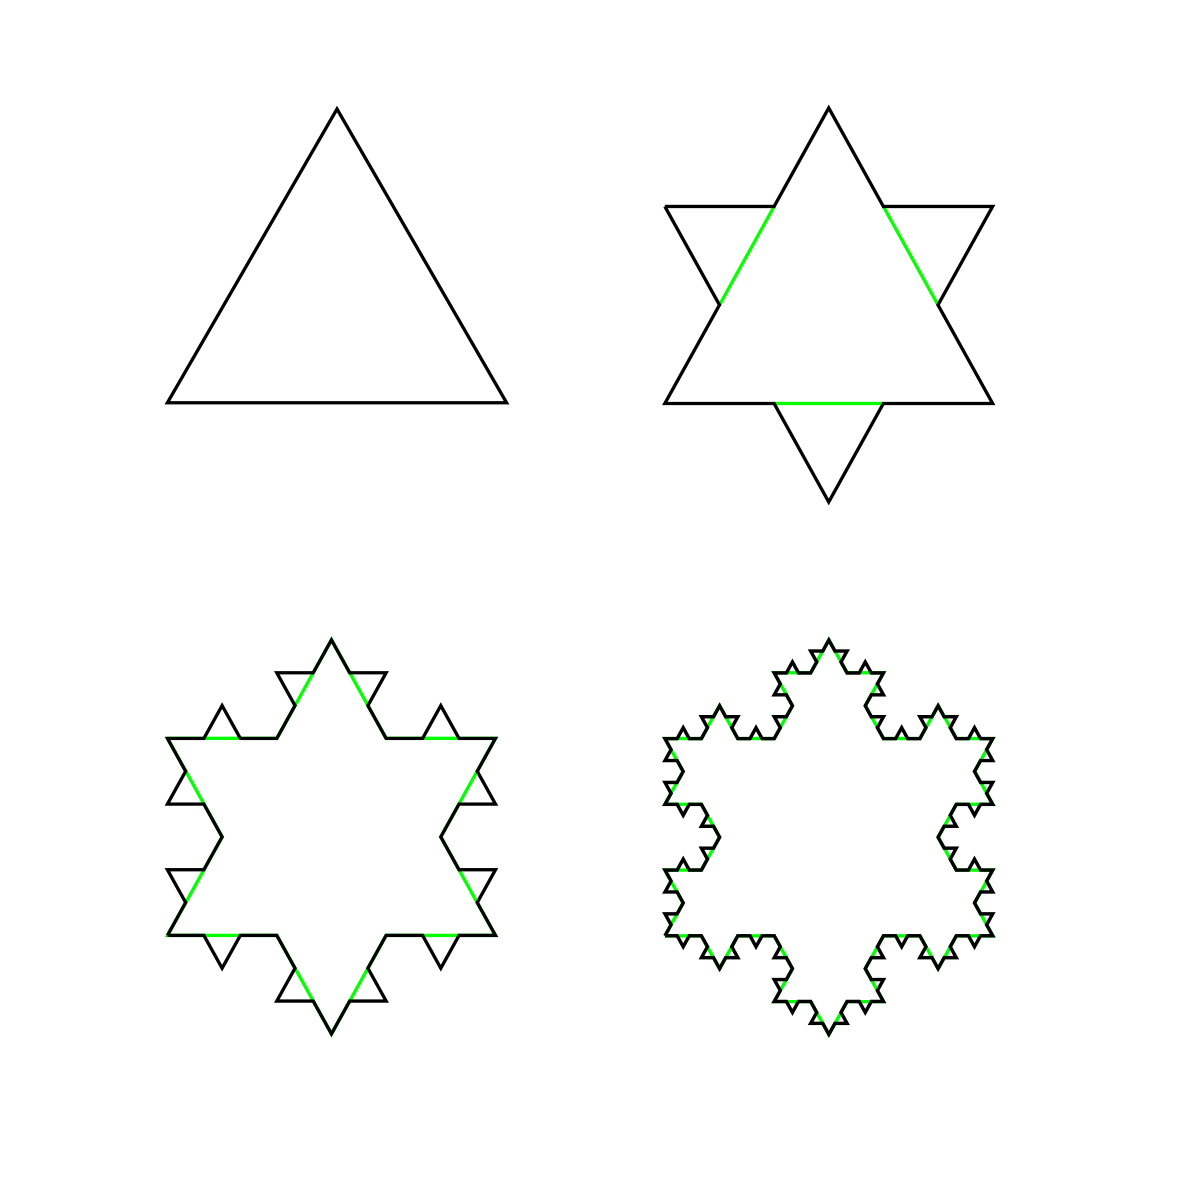
\includegraphics[width = 0.6667\textwidth]{KochFlake}}
\caption{\label{fig:kochflake} Koch snowflake
curve.\protect\footnotemark}
\end{figure}

\footnotetext{Image in \ref{fig:kochflake} licensed Creative
Commons Attribution-ShareAlike 3.0 Unported.}

A paradigmatic method of generating fractals is multiple copy reduction machine
(MCRM). Imagine a copier with more than one lens, each equipped with adjustments
(sliding, shrinking, or rotating the image of the original). Make a copy,
replace the original with the copy, and repeat to infinity. Just as with the
snowflake curve, the final copy comes to occupy a definite fraction of the
picture plane and thus is a fractal \cite{chaosandfractals}.

Mathematically, the MCRM is an iterated function system. Each lens represents an
affine transformation of the plane. Each lens, chosen at random or in turns,
transforms the original set, and the union of the transformations replaces the
original. More formally, an \emph{iterated function system (IFS)} is a
topological space $\mathbb{X}$ with a finite set of continuous functions
$f_{n}:\X\rightarrow \X$, $n=1,2,\dots,N$. If the functions or transformations
are contractive, the Banach Fixed Point Theorem proves that iterating this
mapping to infinity brings the original to a fixed point, the attractor of the
IFS \cite{chaosandfractals, barnsley1985iterated, 10.2307/24893080,
fractalseverywhere}. An \emph{attractor} of the IFS $\cal{F}$ is a set $A\in
\cal{H}(\X)$ the set of all closed compact subsets of $\X$ such that

\begin{enumerate}
\item $\cF(A)=A$, and
\item there is an open set $U\subset \X$ such that $A\subset U$ and
$\lim_{k\rightarrow\infty}\mathcal{F}^{k}(S)=A,$ for all $S\in \cal{H}$ with
$S\subset U$; the limit is with respect to the Hausdorff metric on $\cal{H}$.
\end{enumerate}

\noindent Thus, \textit{any} original will end up producing the
\textit{same} attractor.

Furthermore, Barnsley's Collage Theorem \cite{barnsley:1986:solution} proves
that any original set can be approximated, as closely as desired, by some IFS.

One way this can be done is to cover the attractor with transformed copies of
itself, minimizing overlaps. Let $(\mathbb{X},d_\mathbb{X})$ be a complete
metric space. $(\calH (\X), d_\calH)$ is the associated metric space based on
the hyperspace of nonempty compact subsets of $\X$ with Hausdorff metric
$d_\calH$. Assume $M\in\calH(\X)$ and $\varepsilon > 0$. Assume $\cF := \{\X;
f_1, \ldots, f_N\}$ is a contractive IFS such that

\be\label{hutchop}
d_\calH \left(M, \;\bigcup_{i=1}^N f_i (M) \right) < \varepsilon;
\ee

\noindent the union of contractions is called the \textit{Hutchinson operator}.
Then

\[
d_\calH (M, A) < \frac{\varepsilon}{1-s},
\]

\noindent where $A$ is the attractor of the IFS and  and $s :=
\max\{\mathrm{Lip}\,f_i\st
i = 1, \ldots, N\}$.

\textit{The Collage Theorem is the key motivation for using IFS in music
composition}. The theorem proves that IFS, although conceptually simple, are as
musically powerful as one might like. The remainder of this paper concerns how
to explore the vast parameter space of IFS in a \textit{musically intelligible}
way.

It would be possible to use IFS to generate sound grains on a grid; to generate
notes on a grid; or to generate a path through a different chord space,
\textit{e.g.} use Callender, Quinn, and Tymoczko's $OPC$ instead of $OPTIC$.
Here, we have chosen $OPTIC$ in order to work at the highest level of harmonic
abstraction.

So, we have the harmony of a score as a sequence of points in chord symmetry
space, \textit{i.e.}, the graph of a function of time in that space. Graphs of
functions, \textit{i.e.} fractal approximations, can be computed by a special
kind of IFS associated with a \textit{Read-Bajraktarevi\'c} operator $\Phi$.

Assume a finite family $\{l_n : X\to X \mid n = 1, \ldots, N\}$ of injective
contractions with the following properties:

\begin{align}
&X = \bigcup_{n=1}^N l_n(X);\label{union}\\
&\Int (l_m(X))\cap \Int(l_n(X)) = \emptyset, \quad\forall\;m, n\in \{1,\ldots,
N\}, m\neq n.
\end{align}

\noindent Here, $\Int (S)$ denotes the interior of a set $S$.

Suppose that $(Y,d_Y)$ is a complete metric space with metric $d_Y$. A mapping
$g:X\to Y$ is \emph{bounded} (with respect to the metric $d_Y$) if
there exists an $M > 0$ so that for all $x_1, x_2\in X$, $d_Y(g(x_1),g(x_2)) <
M$. Then the Read-Bajraktarevi\'c operator is

\be\label{RB}
\Phi g (x) := \sum\limits_{n=1}^N F_n (l_n^{-1} (x), g\circ l_n^{-1}
(x))\,\chi_{l_n(X)}(x),
\ee

\noindent where $\chi_M$ is the characteristic function of a set $M$.
Equivalently, \eqref{RB} can be written

\be\label{3.3}
(\Phi g \circ l_n) (x) := F_n (x, g(x)),\quad x\in X, \;n = 1, \ldots, N.
\ee

\noindent Because operator $\Phi$ is well-defined, $g$ is bounded, and each
$v_i$ contractive in the second variable, $\Phi g\in B(X,Y)$.  In other words,
each of the contractions in the RB operator applies to a disjoint subset of the
domain of the bounded mapping, and contracts the range of the mapping. Figure
\ref{fig:fif} shows the graph of a function computed by an RB operator
consisting of three bilinear transformations (in the computer graphics sense,
not the signal processing sense).

\begin{figure}
\centerline{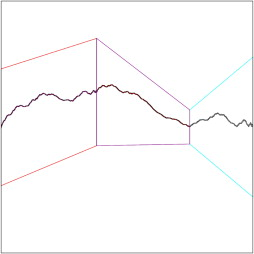
\includegraphics[width = 0.5\textwidth]{interp}}
\caption{\label{fig:fif} Three bilinear transformations in
a fractal interpolation function.\protect\footnotemark}
\end{figure}

\footnotetext{Image in \ref{fig:fif} from \cite{barnsley2015bilinear}.}

The relationship of the RB operator $\Phi$ to the IFS $\cF$ of a score graph
$G$ is shown in this commutative diagram:

% \be\label{Phi}
% \begin{CD}
% X\times Y @>\cF_\Phi>> X\times X\\
% @AAGA                  @AAGA\\
% B(X,Y) @>\Phi>>  B(X,Y)
% \end{CD}
% The commutativity of the diagram (2.13) then holds with F Φ replaced by F and Φ
% replaced by Φ F .
% \ee

\be\label{Phi}
\begin{CD}
X\times Y @>\cF>> X\times X\\
@AAGA                  @AAGA\\
B(X,Y) @>\Phi_\cF>>  B(X,Y)
\end{CD}
\ee

\noindent where $G$ is the mapping $B(X,Y)\ni g\longmapsto G(g) = \{(x,
g(x))\mid x\in X\}\in X\times Y$.

Please recall, here we use the \textit{graph} of a bounded fractal function to
represent the harmonic progression of s musical score, not the fractal function
as such. Our purpose in using the RB operator is to ensure that we specify
\textit{only} IFS that compute harmonic progressions.

The concepts of fractal interpolation and the RB operator carry over to
\textit{local} iterated functions, in which the transformations belonging to the
Hutchinson operator may have different domains although they have the same
co-domain. This provides more flexibility in the construction of FIFs. Assume
that $\X$ is a closed subset of a complete metric space. Consider the complete
metric space $\X\times\Y$ and define mappings $w_i:\X_i\times\Y\to\X\times\Y$ by

\be\label{IfsForFif}
w_i (x, y) := (u_i (x), v_i (x,y)), \quad i\in \N_N.
\ee

In this equation, each $u_i$ maps the \emph{domain} t of the graph to one of the
partitions of the domain, and the $v_i$ are transformations that rescale
the \emph{range} of the graph. If the $v_i$ have the same domain, then we have a
regular IFS; but if the $v_i$ have different domains but the same co-domain,
then the family $\cW_\loc := \{\X\times\Y; (\X_i\times\Y, w_i)\st i\in \N_N\}$
is a contractive \textit{local} IFS in the metric $d_\theta$ and the graph
$G(f^*)$ of the local fractal function $f^*$ associated with the operator $\Phi$
given by \eqref{Phi} is an attractor of $\cW_\loc$. Moreover,

\be\label{GW}
G(\Phi f^*) = \cW_\loc (G(f^*)),
\ee

\noindent where $\cW_\loc$ denotes the Hutchinson operator \eqref{hutchop}
associated with the local IFS $\cW_\loc$. Different transformations may then be
used to transform different partitions of the domain.

In the literature, a variety of transformations have been used for the $v_i$ in
this FIF scheme. For the most part, these reflect the original intention of
interpolating functions to fit existing data points. For the purposes of
adapting this method for musical composition, we adopt from
\cite{2012arXiv1209.3139B} one of the simpler and clearer transformations, the
bilinear transformation, expressed with linear partitions of the domain and a
vector-valued range as:

\be\label{bilinear}
w_{i}(x,\mathbf{y}) :=[x_{i-1} + \frac{x_{i}-x_{i-1}}{x_{N}-x_{0}})
(x-x_{0}),\mathbf{a}_i+\mathbf{b}_ix+\mathbf{c}_i\mathbf{y}+\mathbf{d}_ix
\mathbf{y}],
\ee

\noindent where $x$ is time and $\mathbf{y}$ is a point in chord symmetry space $\{P,
I, T\}$, and so the parameters $\mathbf{a, b, c, d}$ are vector-valued.
As in \cite{2012arXiv1209.3139B}, Equation \eqref{bilinear} is solved for
$\mathbf{a, b, c, d}$ using the interpolation data points to neatly fit together
the sub-domains and ranges (Figure \ref{fig:fif}) with the following
equation, where $x$ is the time dimension of the score graph, $\mathbf{y}$ is
the chord symmetry dimension of the score graph, the $X$ are interpolation
points for time, $\mathbf{Y}$ are vector-valued interpolation points for $\{P,
I, T\}$, and $\mathbf{s}$ are vector-valued scaling factors that ensure
contraction to the fixed point of the attractor, i.e.\ the harmony graph, and
provide some control over the shape of the graph between the interpolation
points:

\begin{align}
w_{i} &  (x,\mathbf{y})= \left(X_{i-1}+ \left(  \frac{X_{i}-X_{i-1}}{X_{N}-X_{0}}\right)
(x-X_{0}),\mathbf{Y}_{i-1}+\left(  \frac{\mathbf{Y}_{i}-\mathbf{Y}_{i-1}}{X_{N}-X_{0}%
}\right)  (x-X_{0})\right.\label{bilinear2}\\
& \left. + \left[  \mathbf{s}_{i-1}+\left(  \frac{\mathbf{s}_{i}-\mathbf{s}_{i-1}}{X_{N}-X_{0}}\right)
(x-X_{0})\right]  \left[  \mathbf{y}-\mathbf{Y}_{0}-\left(  \frac{\mathbf{Y}_{N}-\mathbf{Y}_{0}}{X_{N}-X_{0}%
}\right)  (x-X_{0})\right]\right)  .\nonumber
\end{align}

Note that $N$ interpolation points define $N-1$ transformations in the
Hutchinson operator. The interpolation points $\{I : (X_i, \mathbf{Y}_i,
\mathbf{s}_i) \mid \mathbf{s} \in [0, 1), i \in 0, 1, 2, 3, \dots N\}$ will be
exactly reproduced as specific chords at specific times $X_i$ in the score.
Additional chords may also be generated depending on the scaling factors
$\mathbf{s}_i$, the number of interpolation points, and so on.

\subsection{Using Affine Transformations}

We specify the Hutchinson operator for a score generator by starting with $N$
interpolation points $I_i$ for the time-harmony function, which are entered as
the time and harmony translation elements of $N$ homogeneous affine
transformation matrices. Zeroes are entered for all matrix elements that would
act to rotate in any of the time-harmony planes. The elements of the homogeneity
vector are left unchanged. Any of the other elements may be given any value, as
long as the Hutchinson operator derived from those interpolation points remains
contractive.

\[
  I_i=
  \left[ {\begin{array}{cccccccc}
     & 0 & 0 & 0 &   &   &   & t\\
   0 &   &   &   &   &   &   & P\\
   0 &   &   &   &   &   &   & I\\
   0 &   &   &   &   &   &   & T\\
     &   &   &   &   &   &   &  \\
     &   &   &   &   &   &   &  \\
     &   &   &   &   &   &   &  \\
   0 & 0 & 0 & 0 & 0 & 0 & 0 & 1\\
  \end{array} } \right]
\]

Before applying the Hutchinson operator, the interpolation points are copied to
new homogeneous affine transformation matrices $W_i$, and the elements for
scaling and translating time and harmony in the $W_i$ are derived from the
interpolation points for time and harmony that have been entered in the $I_i$,
according to a modification of Equation \eqref{bilinear2} that omits the scaling
factors (\emph{i.e.}, uses a plain shear transformation instead of the bilinear
transformation). For time-harmony points $(t,\mathbf{h})$, where the harmony
dimensions $\mathbf{h}$ are $\{P, I, T \}$, we constrain the Hutchinson operator
to subdivide the time-harmony planes by time,

\begin{align}
w_{i} &  (t,\mathbf{h})= \left(T_{i-1}+ \left(  \frac{T_{i}-T_{i-1}}{T_{N}-T_{0}}\right)
(t-T_{0}),\mathbf{H}_{i-1}+\left(  \frac{\mathbf{H}_{i}-\mathbf{H}_{i-1}}{T_{N}-T_{0}%
}\right)  (t-T_{0})\right.\label{affine}\\
& \left. +   \mathbf{h}-\mathbf{H}_{0}-\left(  \frac{\mathbf{H}_{N}-\mathbf{H}_{0}}{T_{N}-T_{0}%
}\right)  (t-T_{0})\right)  .\nonumber
\end{align}

\noindent Note that $N-1$ Hutchinson operator transformations are derived from
$N$ interpolation points. Then in matrix $W_i$ the translation of time is
$T_{i-1}$, the scaling of time is $\left(
\frac{T_{i}-T_{i-1}}{T_{N}-T_{0}}\right)$, the translation of harmony is
$\mathbf{H}_{i-1}$, and the scaling of harmony is
$\frac{\mathbf{H}_{i}-\mathbf{H}_{i-1}}{T_{N}-T_{0}}$. In matrix form:

\[
  W_i=
  \left[ {\begin{array}{cccccccc}
  \frac{I_{i,11}-I_{i-1,11}}{I_{N,11}-I_{0,11}}              & 0 & 0 & 0 &   &   &   & I_{i-1,18}\\
   0 & \frac{I_{i,22}-I_{i-1,22}}{I_{N,22}-I_{0,22}}             &   &   &   &   &   & I_{i-1,28}\\
   0 &   & \frac{I_{i,33}-I_{i-1,33}}{I_{N,133}-I_{0,33}}            &   &   &   &   & I_{i-1,38}\\
   0 &   &   & \frac{I_{i,44}-I_{i-1,44}}{I_{N,44}-I_{0,44}}             &   &   &   & I_{i-1,48}\\
     &   &   &   &                                                           &   &   &  \\
     &   &   &   &                                                           &   &   &  \\
     &   &   &   &                                                           &   &   &  \\
   0 & 0 & 0 & 0 & 0                                                         & 0 & 0 & 1\\
  \end{array} } \right].
\]




\subsection{Parametric Maps for Scores}

In order to chart a 2-dimensional, rectangular bounded parametric map over a
range of fractal approximations of score graphs, a simple recursive procedure
may be used. First, we define an order for the parameters on the RHS of
\eqref{bilinear2}: simply $\{X, \mathbf{Y}, \mathbf{s}\}$. Similarly, within
each Hutchinson operator, we order the transformations by the order of their
parameters. The actual ordering is not significant as long as the different sets
of parameters are laid out in the \textit{same} order. Of course, two different
FAs may have different numbers of mappings in their respective Hutchinson
operators. To account for that, we pad the shorter operator with zeros.

We take the smaller of two parameters $W_{min}$ as the upper left corner of the
map, and the larger of the two parameters $W_{max}$ as the lower right corner of
the map. If we define a fixed number on each side of parameter points between
the corners, we may then use simple linear interpolation to calculate any
parameter point between those corners. To do this, we divide up the map between
the corners by $N$ intervals for the two most significant parameters. We then
divide each square in the same way for the next two most significant parameters,
and so on. The score graph is then computed for each of the points in the final
map, the actual score is rendered from the score graph, and the parameter point
is colored by some quantitative feature of the score. Alternatively, a thumbnail
visual rendering of the score, a condensed piano roll, may be used; that is our
approach here.

Needless to say, an arbitrary-precision library for floating-point arithmetic
(such as the GNU MPFR \cite{Fousse:2007:MMB:1236463.1236468}) must be used to
store the virtual parameters, which can encode more information than any native
floating-point number format can contain.

\section{Musical Examples}

\subsection{Parametric Mapping}

\subsection{Interpolating Between Pieces}

\subsection{Using the Genetic Algorithm with Fractal Interpolation
Functions}

\section{Future Directions}

It is interesting that, as Massopust notes \cite{massopust2017}, \begin{quote}D.
Hardin proved in 2012 that every compactly supported refinable function is a
piecewise fractal function. In particular, the unique compactly supported
continuous function determined by the mask of a convergent subdivision scheme is
a piecewise fractal function. \end{quote} This implies that the same technique
of parametric composition based on FAs and described here, would also work for
composing sound directly using refinable sets of sound grains, \textit{e.g.}
wavelets.

It also is interesting that Barnsley, Hegland, and Massopust
\cite{2013arXiv1309.0972B} discuss how to derive fractal approximations of
existing data sets. This implies that it is possible to automatically derive FA
parameters for existing works of note-based music, and then to use the resulting
parameter map or parametric interpolation to analyze the relationship between
the works, or to compose new works intermediate in form between them.

\printbibliography
\end{document}
